\section{Preparando el espacio de trabajo}
Empezamos descargando la imagen ubuntu 20.04 de /href{https://hub.docker.com/_/ubuntu}{Docker Hub}

\begin{figure}[H]
  \centering
  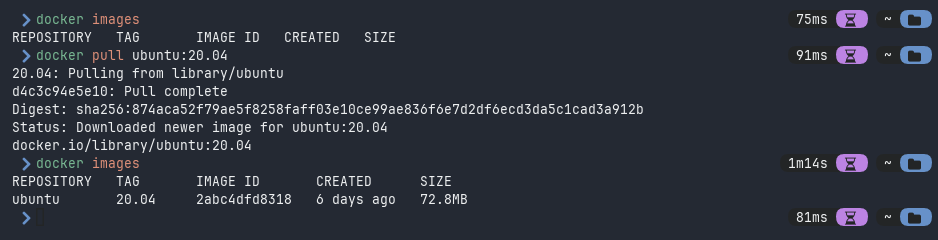
\includegraphics[width=1.0\textwidth]{img/ubuntu_image.png}
  \caption{Instalando la imagen ubuntu:20.04}
\end{figure}

Despues creamos un contenedor a partir de esta imagen y lo iniciamos inmediatamente. Podemos lograr hacer 
esta acciones por separado usando los comandos \textit{create} y seguidamente \textit{start}. Sin embargo 
al no ejecutar nada dentro del contenedor, este se detendrá inmediatamente. 
\singlespacing
Para el primer inicio del contenedor, podemos usar el comando \textit{run}, aprovechando tambien realizar
el \textbf{Port Mapping} de la maquina host a los puertos del contenedor. Tambien para poder interactuar 
con el contenedor le pasamos los argumentos \textit{-it} para  que habra una terminal iterativa y dentro 
de esta ejecutamos el inteprete de comandos \textit{/bin/bash}

\begin{figure}[H]
  \centering
  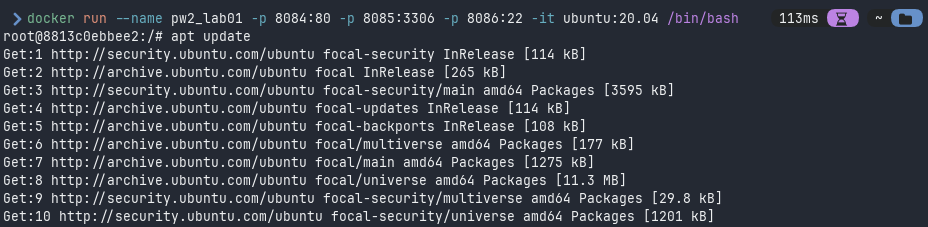
\includegraphics[width=1.0\textwidth]{img/run_container.png}
  \caption{Creando y ejecutando el contenedor}
\end{figure}

Ahora procedemos ha hacer la instalación de un editor de texto necesario para editar código (neovim), un 
servidor web que implemente el protocolo HTTP y HTTPS (Apache), unos lenguajes de scripting (perl, python), 
un sistema de gestion de base de datos (MariaDB) y finalmente un programa servidor que implemente el 
protocolo SSH (openssh)

\begin{figure}[H]
  \centering
  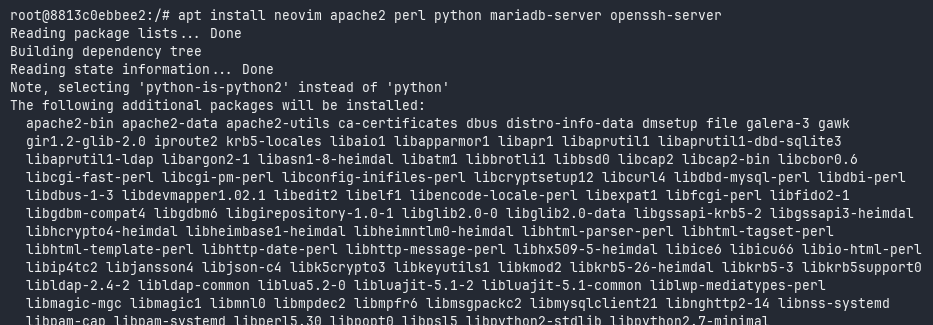
\includegraphics[width=1.0\textwidth]{img/install_programs.png}
  \caption{Instalando los programas para crear y administrar nuestra servidor web}
\end{figure}

Verificamos que la instalación haya sido un exito

\begin{figure}[H]
  \centering
  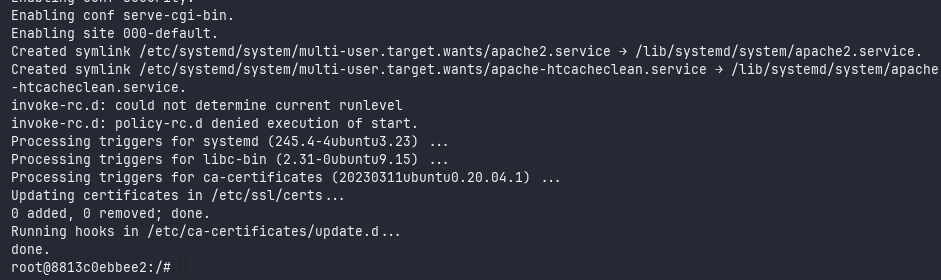
\includegraphics[width=1.0\textwidth]{img/check_install.png}
  \caption{La instalación ha sido un éxito}
\end{figure}

Podemos verificar el estado de los programas servidor que hemos instalado, estos servicios son bien conocidos 
como \textbf{Demonios} ya que son bucles infinitos, que siempre estan escuchando. Los servidores siempre se 
deben de activar. Incluso podemos configurar su activación automatica cuando arranque el sistema operativo.

\begin{figure}[H]
  \centering
  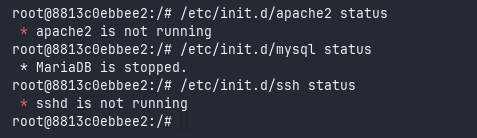
\includegraphics[width=0.6\textwidth]{img/check_daemons.png}
  \caption{Estado de los programas servidor}
\end{figure}

Por el momento solo vamos a iniciar el servidor web Apache y el sistema de gestion de base de datos MariaDB.

\begin{figure}[H]
  \centering
  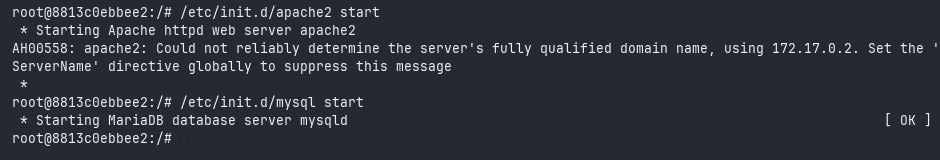
\includegraphics[width=1.0\textwidth]{img/start_daemons.png}
  \caption{La instalación ha sido un éxito}
\end{figure}

Podemos probar el funcionamiento del servidor web de nuestro contenedor en nuestro navegador de nuestra 
maquina host poniendo la direccion IP del contenedor, o simplemente instalando y usando el programa 
\textir{curl} que es una herramienta en la terminal.

\begin{figure}[H]
  \centering
  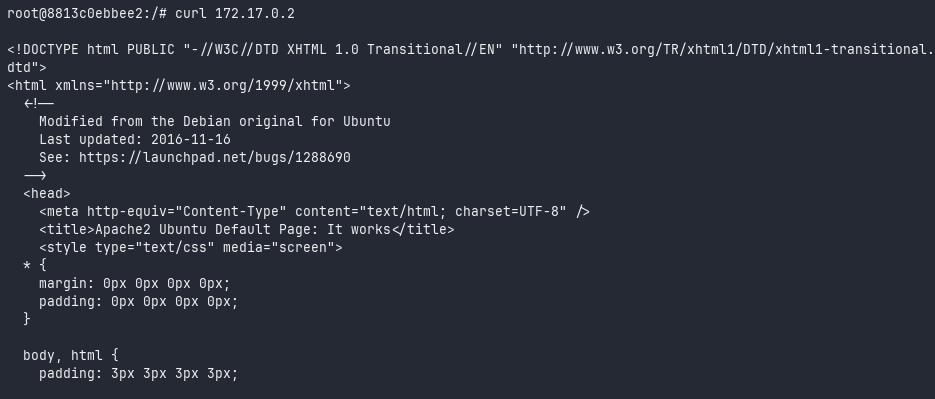
\includegraphics[width=1.0\textwidth]{img/server.png}
  \caption{Archivo \textit{index.html} ubicado en el directorio por defecto \textit{/var/www/html}}
\end{figure}

Bien, seguimos con la configuración de los directorios por defecto en los cuales Apache escucha las 
solicitudes por defecto. Es un mala práctica que se use el directorio por defecto \textit{/var/www/html}. 
Siempre se ha recomendado crear tu propio directorio y como root poder restringir el acceso según 
el contexto.
\singlespacing
Ahora vamos a configurar el servidor web Apache para que pueda ejecutar CGI's. Apache trae consigo dos 
modulos nativos \textit{mod-cgi} y \textit{mod-cgid}. Además la ejecución solo se dá en el directorio 
\textit{/lib/cgi-bin}
\singlespacing
Vamos a crear un test en Python para ver el funcionamiento. Una vez que creamos el archivo .py, tenemos 
que otorgarle el permiso de ejecución, ya que es un script que Apache debe de ejecutar.

\begin{figure}[H]
  \centering
  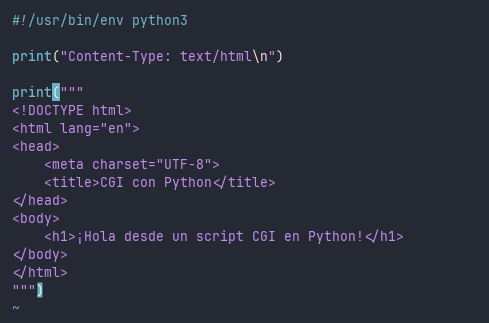
\includegraphics[width=0.6\textwidth]{img/create_cgi.png}
  \caption{Archivo en \textit{/lib/cgi-bin/test.py} y otorgar permisos}
\end{figure}

\begin{figure}[H]
  \centering
  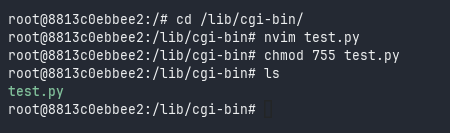
\includegraphics[width=0.6\textwidth]{img/cgi_with_python.png}
  \caption{CGI con python}
\end{figure}

\begin{figure}[H]
  \centering
  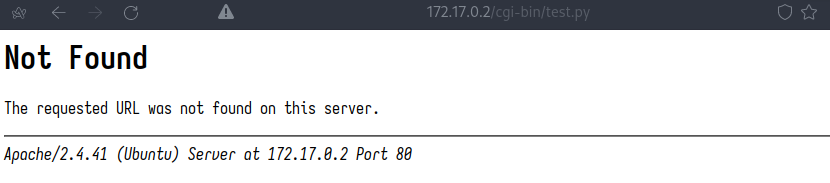
\includegraphics[width=1.0\textwidth]{img/test_error.png}
  \caption{Apache solo escucha en \textit{/var/www/html}}
\end{figure}

Como vemos falta hacer alguna configuracion para que Apache pueda realizar esta funcionalidad. De hecho, 
debemos de habilitar los modulos CGI. Una vez activado el modulo, nosotros debemos de reiniciar Apache.

\begin{figure}[H]
  \centering
  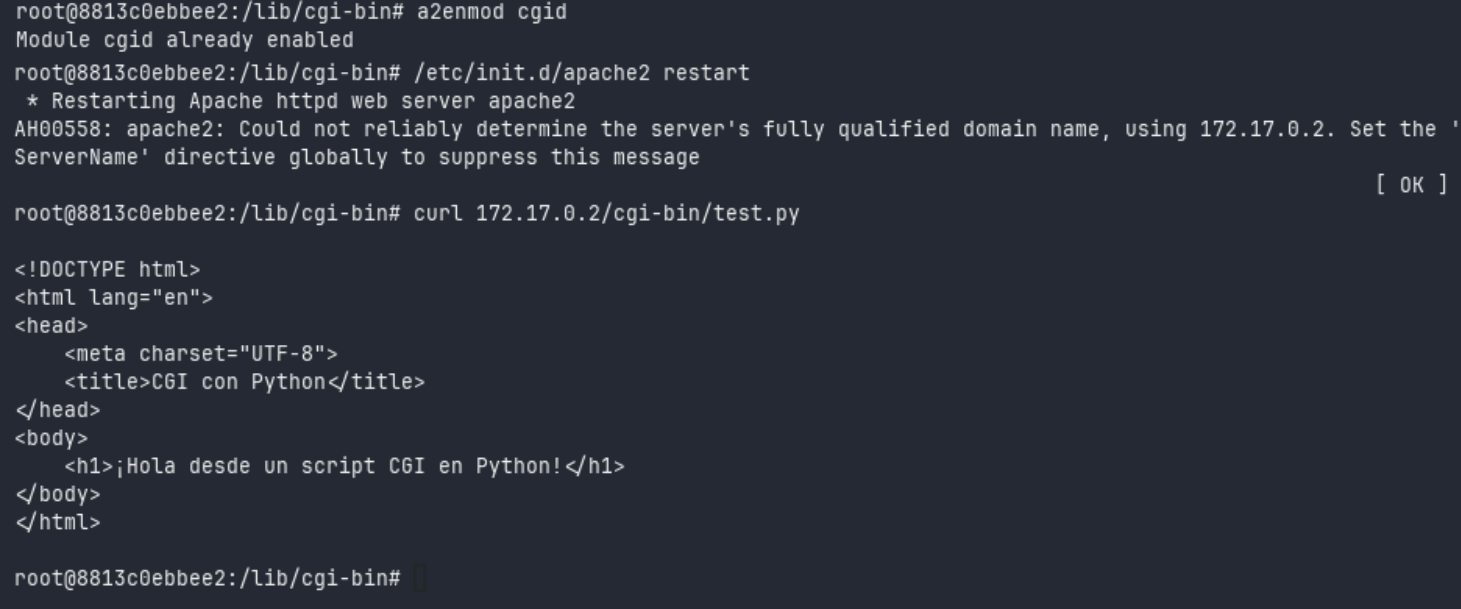
\includegraphics[width=1.0\textwidth]{img/restart.png}
  \caption{Reiniciar el servidor}
\end{figure}

Ahora si podemos estar seguros que los CGIs se van a ejecutar

\begin{figure}[H]
  \centering
  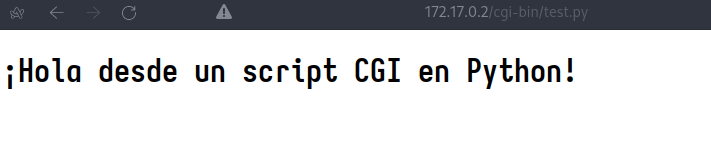
\includegraphics[width=1.0\textwidth]{img/test.png}
  \caption{Test exitoso}
\end{figure}

\subsection{Cambiando a directorios personalizados}
Para hacer los cambios, nosotros debemos modificar los archivos de configuración de apache. Apache 
maneja el concepto de Virtual Host que nos permite tener varias aplicaciones web en solo un servidor 
web fisico. Esto se logra configurando Apache para que responda a diferentes nombres de dominio (o direcciones IP) y sirva contenido específico para cada uno de ello.\\

Las bloques de configuracion que vamos a realizar van a definir el nombre de dominio, el directorio raiz y 
otras opciones de configuracion. Lo que vamos a hacer es crear un archivo \textit{/etc/apache2/sites-available/aplicaciones\_web} y aqui colocamos las configuraciones.

\begin{figure}[H]
  \centering
  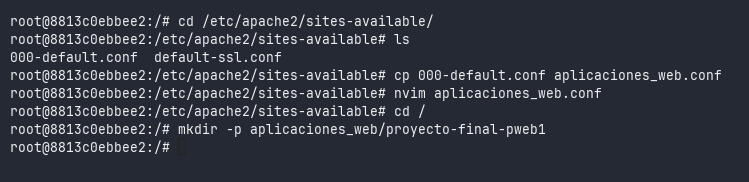
\includegraphics[width=0.8\textwidth]{img/directories.png}
  \caption{Creación del archivo de configuración}
\end{figure}

\begin{figure}[H]
  \centering
  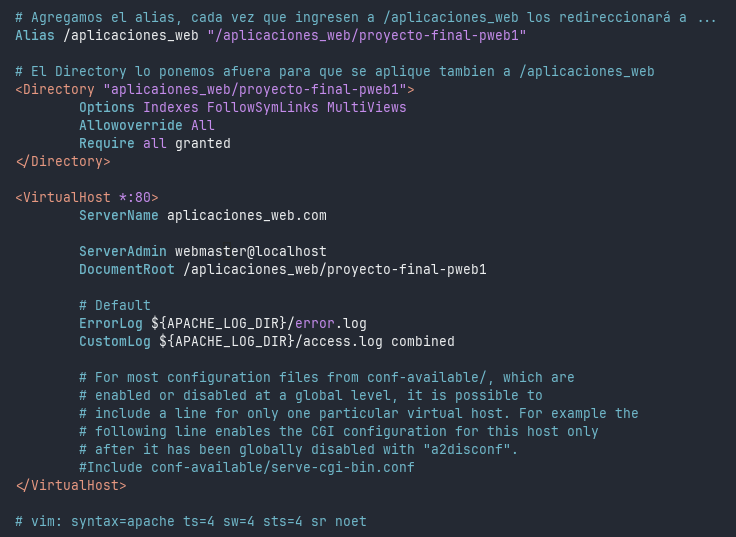
\includegraphics[width=0.8\textwidth]{img/conf.png}
  \caption{configuración del Virtual Host}
\end{figure}

Una vez que hicimos las respectivas configuraciones, ahora necesitamos activar el sitio web, activamos el modulo \textbf{mod-rewrite} que se encarga de realizar las redirecciones de solicitudes.

\begin{figure}[H]
  \centering
  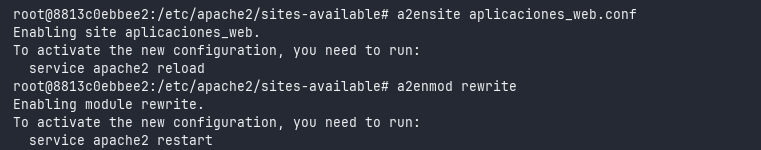
\includegraphics[width=0.8\textwidth]{img/enable_conf.png}
  \caption{Habilitamos el sitio web configurado}
\end{figure}

Ahora necesitamos que los CGIs se utilicen en directorios especificos. Para ello nosotros nos vamos al 
directorio \textit{/etc/apache2/conf-available} donde vamos a crear una configuración para que apache pueda 
ejecutar los CGIs en el directorio, por ejemplo, \textit{/aplicaciones\_web}

\begin{figure}[H]
  \centering
  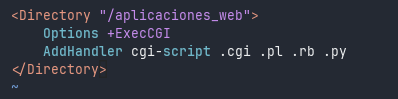
\includegraphics[width=0.6\textwidth]{img/cgi_conf.png}
  \caption{Archivo de configuración}
\end{figure}

Por ultimo habilitamos la configuración y como siempre, reiniciamos el servidor Apache

\begin{figure}[H]
  \centering
  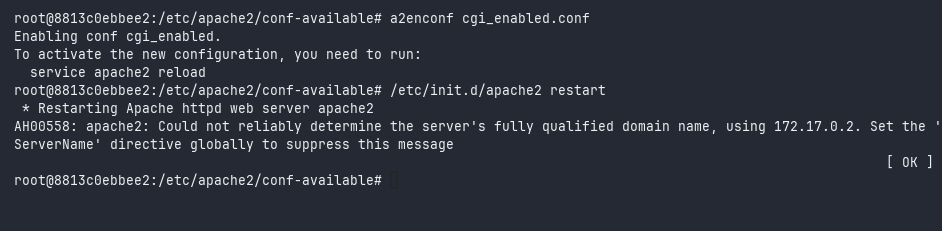
\includegraphics[width=1.0\textwidth]{img/restart2.png}
  \caption{Habilitando las configuración}
\end{figure}




